\tightsection{Challenges of Practical Prediction Algorithms}
\label{sec:challenges}

While in previous section we showed that video metrics are predictable with the attributes we chose, there are still several practical challenges in designing such prediction algorithm. 

The most straightforward and naive prediction algorithm is take the mean of quality samples from the sessions that match all attributes to the session under prediction.
This naive algorithm faces the following challenge: while the potential of the algorithm increases with more attributes, the data points (quality samples) contained in each fine-grained identical group\footnote{In the case of quality sample, an identical group consists of quality samples whose session matches all value in an AC.} becomes {\it sparse}, and such sparsity is susceptible to noise. Moreover, a practical algorithm inherently has a processing delay so that the session under prediction can only be predicted using information that was collected a while ago.

%\xil{the following seems to be only part of the challenge}
%In particular, a practical algorithm can only use the information (quality samples) collected before the minute that the session under prediction belongs to.

This section first categorizes the sources of difficulty in predicting video quality accurately (\Section~\ref{subsec:challenges}) which informs the choice of aggregating identical groups of all attributes (i.e., the finest identical groups) by ignoring (hopefully, less important) attributes so that more samples will be used (\Section~\ref{subsec:aggregation}) to counteract the noise and estimation error brought by sparse data.

\tightsubsection{Sources of prediction error}
\label{subsec:challenges}
%Although the figures~\ref{fig:predictability} show that in many cases, quality is similar among quality samples that share the same attribute values and same temporal interval, there are still a lot of quality sample groups that have high dispersion. This is one of the key challenges that make quality prediction difficult. 
%In this part, we enumerate the potential reasons that causes the dispersion we observe. Intuitively, if the number of similar sessions is small (e.g., $~10$ sessions), the mean quality outcome is subject to considerable random noise.  If we use this mean for prediction, the prediction will be subject to the same noise and consequently to high average error.  As the number of attributes grows, quality grows more predictable (as the noise decreases) but the number of perfectly-matched sessions may drop exponentially.

%Of course, prediction in the presence of limited information is statistics problem, and there are many potential solutions to this problem.  
In general, there are four sources of prediction error:
%Any solution will deal with, and potentially trade off, four sources of prediction error:

\begin{packedenumerate}
  \item \emph{Estimation error} caused by limited data.  Even other things being equal, more data produce more accurate prediction. For example, Figure~\ref{fig:group-size-impact} presents the prediction error vs. group size (i.e., number of samples). Given a large number of attributes and the combinatorial nature of the attributes (the number of groups grow exponentially with more attributes), estimation error is a serious problem in practice. 
  % Using all available attributes, many sessions have very few matches, as we would expect given the exponential explosion in combinations of attribute values.  

\begin{figure}[h!]
\centering
\subfigure[Prediction error vs. group size (w.r.t average bitrate)]
{
        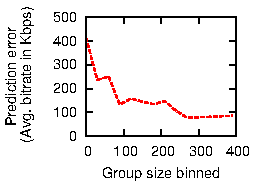
\includegraphics[width=110pt]{figures/count-err.pdf}
	\label{subfig:group-size-impact:count-err}
}
\subfigure[Distribution of group size]
{
        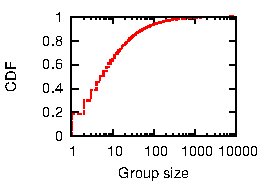
\includegraphics[width=110pt]{figures/count-cdf.pdf}
}
\tightcaption{Impact of group size (i.e., number of samples in a group). They show that more samples give more accuracy, but most of groups do not have sufficient samples for accurate prediction.}
\label{fig:group-size-impact}
\end{figure}

\item \emph{Bias} due to missing or unused information: The bias occurs when we do not observe (or use) an attribute that is important for prediction. Bias is not alleviated by gathering data from more session, but by gathering more attributes from each session.

\item \emph{Unavailability of recent data:} In a practical system, there are delays in measuring, sending and processing quality samples, so they are not available instantly.  If conditions change rapidly, there may be no quality samples sufficiently close to the session under prediction.  This is an extreme example of estimation error.  In this case it may be necessary to model the evolution of the video ecosystem over time in order to extrapolate to the current time. Figure~\ref{fig:quality-variability} shows per-minute quality variability. It shows that even with sufficient data, the mean value of a group of quality samples could vary significantly. This clearly indicates that any practical algorithm has to be running in real-time (on the order of one minute or less).

\begin{figure}[h!]
\centering
 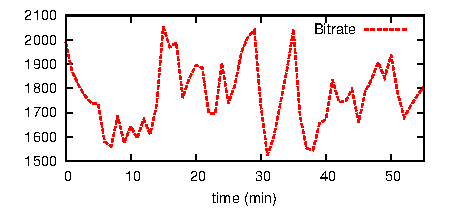
\includegraphics[width=0.4\textwidth] {figures/quality-time.pdf}
\tightcaption{Temporal variability of quality. The figure shows the mean value of average bitrate of a fixed group of same [Site, Initial CDN, Initial Bitrate, ConnectionType, ASN, Object], which has 100 quality samples in every minute in the figure.}
\label{fig:quality-variability}
\end{figure}

  \item \emph{Noise:} Even if we observed all conceivable attributes of a session and had infinitely many examples of exactly quality samples, outcomes may be affected by non-deterministic inputs.  For example, performance may be affected by exponentially backoff at the data link layer or the congestion generated by cross traffic at the network layer. This implies that some degree of prediction error is inevitable.
\xil{can i say this is Bias? because we do not capture this feature, and it is hard for us to extract a feature out of it, we consider it as noise?}
\end{packedenumerate}

%\xil{need a conclusion.}\jc{don't have a good conclusion to put here. we have to at least claim that fixing estimation error is feasible based on our algorithm.}

Thus for any practical algorithm, it is a challenge to manage prediction error, which we will elaborate in the following section.

\comment{
\begin{align}
  \label{eqn:biasvariance}
  \E_D[(p_i - q_i)^2] &= \Var_D[p_i - q_i] + (\E_D[p_i - q_i])^2
\end{align}
\begin{align*}
  \label{eqn:biasvariancelong}
  &= \Var_D[p_i - \hat{q}_i - \epsilon_i] + (\E_D[p_i - \hat{q}_i - \epsilon_i])^2 \\
  &= \Var_D[p_i - \hat{q}_i] + \Var_D[\epsilon_i] + (\E_D[p_i - \hat{q}_i - \epsilon_i])^2\\
  &= \Var_D[p_i] + \Var_D[\epsilon_i] + (\E_D[p_i - \hat{q}_i - \epsilon_i])^2\\
  &= \Var_D[p_i] + \Var_D[\epsilon_i] + (\E_D[p_i - \hat{q}_i] - \E_D[\epsilon_i])^2\\
  &= \Var_D[p_i] + \Var_D[\epsilon_i] + (\E_D[p_i] - \hat{q})^2
\end{align*}
}

%The first term in equation \eqref{eqn:biasvariancelong} is estimation error -- the variability in predictions across possible sets of observed data.  It will increase as the number of sessions similar to session $i$ in $D$ decreases. As a special case, it may be very large if only a few quality samples in $D$ are temporally close to session $i$.  The second term is noise.  The third term is the squared bias of the predictor, which does not generally decrease with the size of $D$.  The average prediction error is simply the average over all these three terms of sessions $i$. 

\tightsubsection{Aggregation}
\label{subsec:aggregation}
A simple strategy to reduce estimation error is {\it aggregation}.  By aggregation we mean putting quality samples into coarser groups that match on only a subset of observed attributes.  Aggregation increases the number of samples in each identical group by reducing the number of attributes, thus reducing estimation error at the cost of increased bias. 
Intuitively, when estimation error is small (say, when a fine-grained identical group contains many sessions) we want to eliminate bias by using a fine-grained group.  When estimation error is large, we want to aggregate more. 
Then the question becomes how to determine the best level of aggregation.


\begin{figure}[h!]
\centering
 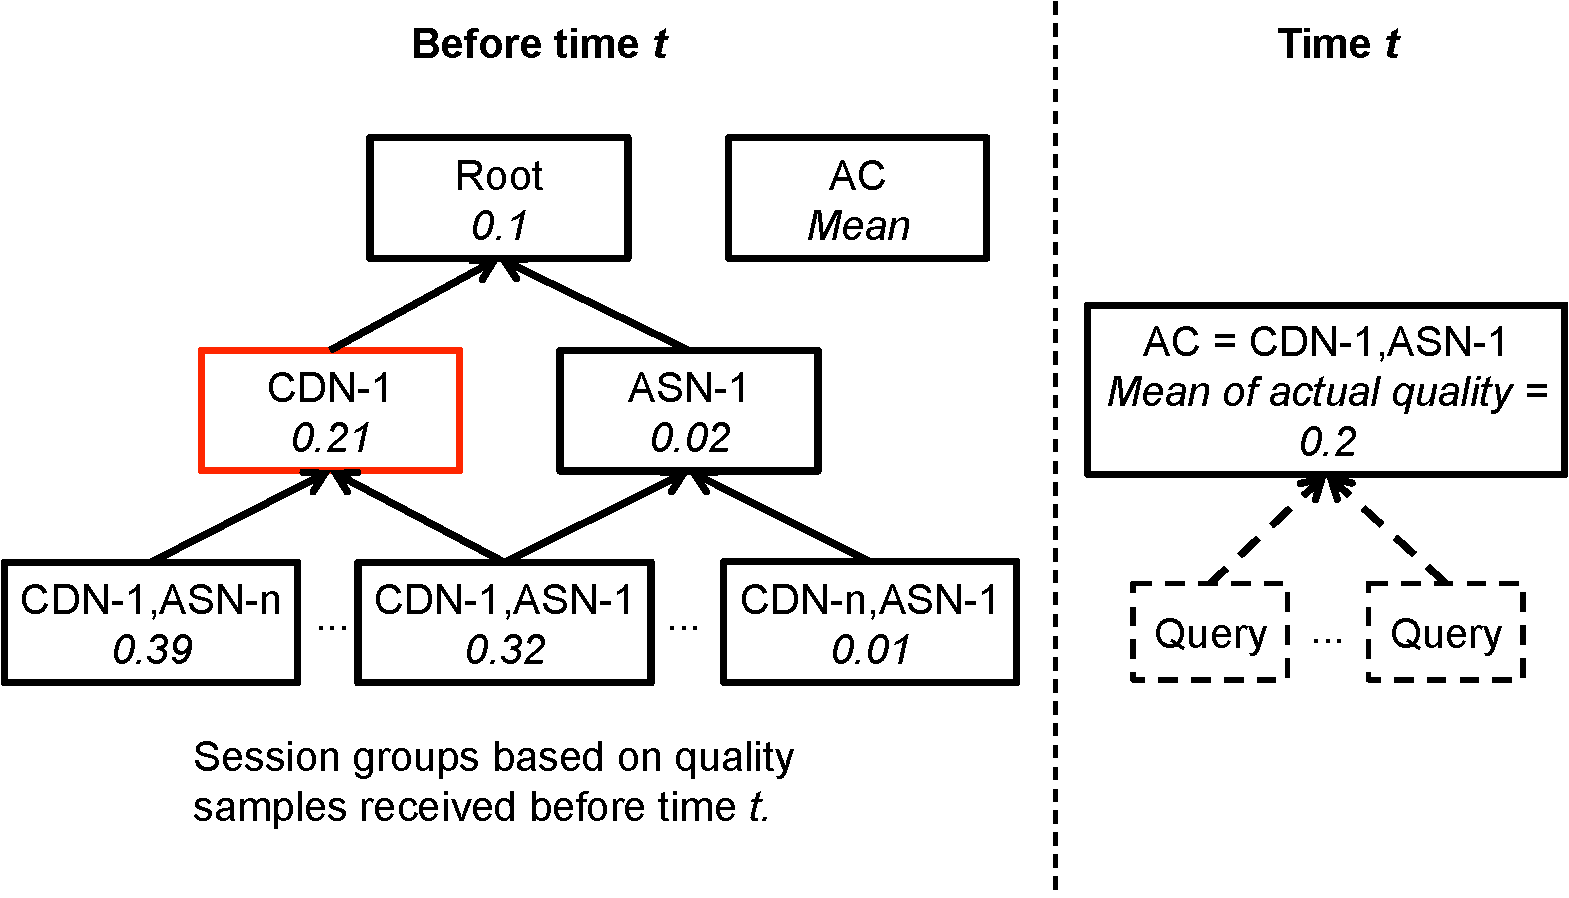
\includegraphics[width=0.5\textwidth] {figures/fig-optimal-AC.pdf}
\tightcaption{Example of how optimal AC is identified. The optimal AC is colored in red. The optimal AC for an identical group of sessions under prediction is the one of which the mean minimizes the prediction error.}
\label{fig:example-optimal-ac}
\end{figure}

\myparatight{Optimal AC} We use a simple oracle methodology, called {\it optimal AC}, to show the dynamics of the best level of aggregation. We assume an prediction algorithm with a delay of one minute, i.e., it predicts with information (quality samples) collected from previous minute.

Figure~\ref{fig:example-optimal-ac} shows an example of optimal AC with three attributes. For a finest identical group (e.g., $[CDN1,ASN1,Site1]$) at $t$-th minute, we first build a hierarchy that consists of all degrees of aggregation over the quality samples we collects before the $t$-th minute (e.g., the left part of Figure~\ref{fig:example-optimal-ac}). 
Remember that the optimal prediction of this identical group is its mean (see \Section~\ref{subsec:lowerbound}). 
Then, the optimal AC for this identical group is the degree of aggregation that gives the prediction value closest to the optimal prediction for the finest identical group at $t$-th minute. 
For instance, in Figure~\ref{fig:example-optimal-ac}, if the optimal prediction of the targeted identical group is 0.2, the optimal AC (colored in red) is the one with the closest prediction to 0.2, i.e., $(ASN, CDN)$. 


\begin{figure}[h!]
\centering
\subfigure[Distribution of coverage of top five optimal ACs (w.r.t averge bitrate).]
{
        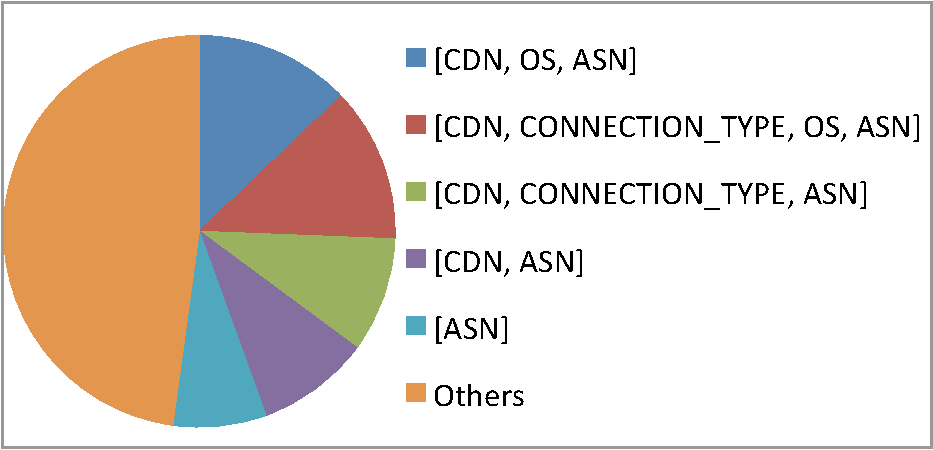
\includegraphics[width=0.4\textwidth]{figures/optimal_AC_distribution.pdf}
}
\subfigure[Optimal AC prevalence.]
{
        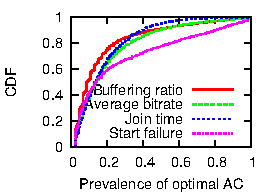
\includegraphics[width=0.24\textwidth]{figures/optimal-prevalence.pdf}
}
\hspace{-0.6cm}
\subfigure[Optimal AC persistence.]
{
        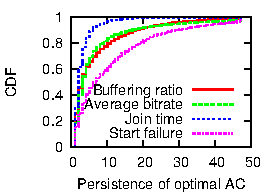
\includegraphics[width=0.24\textwidth]{figures/optimal-persistence.pdf}
}
\tightcaption{Dynamics of the optimal AC. (a) gives coverage of optimal ACs (for each AC, the fraction of sessions of which this AC is the optimal AC).
(b) gives prevalence of pair of (session under prediction, optimal AC) (the fraction of time that the finest group has this optimal AC).
(c) gives persistence of pair of (session under prediction, optimal AC) (i.e., the longest continuous duration where a finest group has the same optimal AC).}
\label{fig:optimal-ac-dynamics}
\end{figure}

To show the dynamics of optimal AC, we present some empirical analysis results over our dataset from three aspects. 
 
\begin{packeditemize}
	\item {\it No single optimal AC:} Figure~\ref{fig:optimal-ac-dynamics}-(a) shows the coverage of optimal ACs, i.e., the fraction of time for which a given AC is the optimal AC. Note that there is no single optimal AC. For example, the finest group only has coverage about 20\% and no coarsest grain AC (single attribute) is among the top 5. This implies that the optimal AC is often in between.
	\item {\it No temporally prevalent optimal AC:} Figure~\ref{fig:optimal-ac-dynamics}-(b) shows the prevalence of the $($\emph{session-under-prediction, optimal AC}$)$ pairs, i.e., the fraction of time the fines group of sessions has the same optimal AC. Note that $70\%$ pairs only last for less than $20\%$ of time. This implies that there is no single or a small set of optimal ACs that can cover most sessions.
	\item {\it Highly dynamic optimal ACs:} Figure~\ref{fig:optimal-ac-dynamics}-(c) shows the persistence of the $($\emph{session-under-prediction, optimal AC}$)$ pairs, i.e., the longest continuous duration where the finest group has the same optimal AC. Only 40\% of pairs last for more than 10 minutes. This suggests that even with a reactive strategy will be challenging to track the optimal ACs.
\end{packeditemize}

To conclude, we find that the optimal AC (the aggregation that gives minimal prediction error) is in many cases neither the finest nor the coarsest one, and, in addition, is highly dynamic. This presents a challenge in designing a practical prediction algorithm to identify the best AC in real-time.
\xil{It is not clear from first read that optimal AC is an oracle analysis, not a real algorithm}

